\documentclass[11pt,a4paper,oneside]{article}
\usepackage[utf8]{inputenc}
\usepackage[margin=1in]{geometry}
\usepackage{graphicx}
\usepackage{amsmath,amsfonts,amssymb}
\usepackage{hyperref}
\usepackage{booktabs,longtable}
\usepackage{tikz}
\usetikzlibrary{shapes,arrows,positioning,calc,decorations.pathmorphing,backgrounds,fit,shadows}
\usepackage{listings}
\usepackage{xcolor}
\usepackage{fancyhdr}
\usepackage{enumitem}
\usepackage{float}

\lstset{
    basicstyle=\ttfamily\small,
    commentstyle=\color{gray},
    keywordstyle=\color{blue},
    breaklines=true,
    numbers=left,
    numbersep=5pt,
    showstringspaces=false,
    tabsize=2
}

\pagestyle{fancy}
\fancyhf{}
\fancyhead[L]{Software Design Document: E-commerce Platform}
\fancyhead[R]{Version 1.0}
\fancyfoot[C]{\thepage}

\hypersetup{
    colorlinks=true,
    linkcolor=blue,
    urlcolor=cyan,
    pdftitle={Comprehensive Software Design Document: E-commerce Platform},
    pdfauthor={AI System Architect},
    pdfsubject={Software Architecture}
}

\title{\Huge\textbf{Comprehensive Software Design Document: E-commerce Platform}}
\author{\Large AI System Architect}
\date{\Large\today}

\begin{document}

\maketitle
\thispagestyle{empty}
\vfill

\begin{center}
\large
\begin{tabular}{|l|l|}
\hline
\textbf{Document Version} \& 1.0 \\
\hline
\textbf{Creation Date} \& \today \\
\hline
\textbf{Document Status} \& Final Draft \\
\hline
\textbf{Generated By} \& AI System Architect \\
\hline
\textbf{Target Audience} \& Development Team, Stakeholders \\
\hline
\textbf{Classification} \& Internal Use \\
\hline
\end{tabular}
\end{center}

\newpage
\tableofcontents
\newpage
\listoffigures
\newpage

\section{Executive Summary}

This document outlines the design for a new e-commerce platform, codenamed "Project Phoenix."  Project Phoenix aims to provide a robust, scalable, and secure online marketplace for businesses to sell their products and services. The platform will leverage a microservices architecture, utilizing cloud-native technologies for deployment and scalability. Key features include user authentication and authorization, product catalog management, shopping cart functionality, order processing, payment gateway integration, and robust reporting capabilities. The business objectives are to increase market share, improve customer satisfaction, and streamline operational efficiency.  The technical approach focuses on modularity, maintainability, and scalability to accommodate future growth.  Key benefits include increased agility in development, improved performance, and enhanced security. The estimated implementation timeline is 6 months, divided into three phases:  design and development, testing and quality assurance, and deployment and launch.

\subsection{Project Scope and Objectives}

Project Phoenix will encompass the development of a complete e-commerce platform, including frontend user interfaces (web and mobile), backend services, and a robust database infrastructure. The platform will support various payment gateways, offer multiple shipping options, and provide comprehensive customer support features.  The primary objectives include:

* **Increase Sales:**  A 20\% increase in sales within the first year of operation.  This will be measured by tracking total revenue generated through the platform.
* **Improve Customer Satisfaction:** Achieve a customer satisfaction rating (CSAT) of 4.5 out of 5 stars based on post-purchase surveys.
* **Enhance Operational Efficiency:** Reduce order processing time by 15\% compared to existing manual processes. This will be monitored through key performance indicators (KPIs) like average order fulfillment time.
* **Expand Market Reach:** Attract 5,000 new businesses to the platform within the first year.  This will be measured by the number of registered vendors.
* **Ensure Platform Scalability:** The platform must be able to handle peak loads during promotional periods and holiday seasons without performance degradation.  This will be evaluated through load testing and performance benchmarks.

Success will be determined by achieving these objectives within the allocated budget and timeline.  Regular progress reports and monitoring of KPIs will be crucial for tracking progress and making necessary adjustments.

\subsection{Key Stakeholders and Roles}

Several key stakeholders will be involved in Project Phoenix:

* **Business Owners:**  Define the business requirements and provide feedback on the platform's functionality.
* **Marketing Team:**  Responsible for promoting the platform and attracting new users and vendors.
* **Development Team:**  Responsible for designing, developing, and testing the platform.  This includes frontend, backend, and database developers.
* **Operations Team:**  Responsible for deploying, monitoring, and maintaining the platform.
* **Customer Support Team:**  Responsible for providing assistance to users and vendors.
* **Security Team:**  Responsible for ensuring the security and integrity of the platform.

\section{Requirements Analysis and Specification}

\subsection{Extracted Requirements Summary}
The initial document provided no specific requirements.  Therefore, this section will be populated with realistic requirements for an e-commerce platform.

\subsection{Functional Requirements}

1. **User Registration and Authentication:** Users should be able to create accounts, log in securely, and manage their profile information.
2. **Product Catalog Management:** Vendors should be able to add, edit, and delete products, including images, descriptions, and pricing.
3. **Shopping Cart Functionality:** Users should be able to add products to their shopping cart, update quantities, and remove items.
4. **Order Placement and Processing:** Users should be able to place orders, select shipping options, and provide payment information.
5. **Payment Gateway Integration:**  The platform should integrate with multiple payment gateways (e.g., Stripe, PayPal) to provide secure payment processing.
6. **Order Tracking:** Users should be able to track the status of their orders.
7. **Inventory Management:**  The system should automatically update inventory levels upon order placement.
8. **Customer Support:**  The platform should provide multiple channels for customer support (e.g., email, chat).
9. **Reporting and Analytics:**  The platform should provide reporting dashboards for sales, inventory, and customer behavior.
10. **Vendor Management:**  Vendors should be able to manage their product listings, orders, and financial information.

\subsection{Non-Functional Requirements}

* **Performance:** The platform should have a response time of less than 2 seconds for most user actions.
* **Scalability:** The platform should be able to handle 10,000 concurrent users and 1,000 orders per minute during peak hours.
* **Security:** The platform should comply with industry best practices for data security and protect against common vulnerabilities such as SQL injection and cross-site scripting (XSS).
* **Availability:** The platform should have a 99.9\% uptime.
* **Maintainability:** The platform should be designed for easy maintenance and updates.
* **Usability:**  The platform should be intuitive and easy to use for both users and vendors.

\section{System Architecture and Design}

\subsection{Architecture Overview}

Project Phoenix will adopt a microservices architecture, deploying each service independently. This allows for greater flexibility, scalability, and maintainability compared to a monolithic architecture.  Each microservice will be responsible for a specific business function, such as user authentication, product catalog management, or order processing.  This modular approach enables independent scaling of individual services based on demand, improving resource utilization and overall platform performance.  The services will communicate with each other through a lightweight message broker (RabbitMQ) and a well-defined API gateway.  This architecture allows for technology diversity, allowing us to choose the best tools for each service.

\begin{figure}[H]
\centering
\begin{tikzpicture}[
    node distance=1cm and 1.5cm,
    font=\sffamily\small,
    base/.style={draw, text width=3cm, minimum height=1.2cm, text centered, rounded corners, drop shadow},
    user/.style={base, fill=Azure!30, text width=2cm},
    api/.style={base, fill=LimeGreen!20},
    service/.style={base, fill=SkyBlue!20},
    database/.style={cylinder, shape border rotate=90, aspect=0.25, draw, fill=Thistle!40, minimum height=1.5cm, text width=2.5cm, text centered, drop shadow},
    external/.style={base, fill=Gold!30},
    arrow/.style={-Stealth, thick, draw=black!60}
]

\node[user] (user) {User};
\node[api, below=1.5cm of user] (gateway) {API Gateway};
\node[service, below=of gateway, xshift=-3cm] (auth) {Authentication Service};
\node[service, below=of gateway] (catalog) {Product Catalog Service};
\node[service, below=of gateway, xshift=3cm] (order) {Order Management Service};
\node[database, below=2cm of auth] (userdb) {User Database (PostgreSQL)};
\node[database, below=2cm of catalog] (productdb) {Product Database (MongoDB)};
\node[database, below=2cm of order] (orderdb) {Order Database (MySQL)};
\node[external, right=2cm of catalog] (payment) {External Payment Gateway};

\begin{scope}[on background layer]
\node[draw, dashed, rounded corners, fill=gray!5, inner sep=0.7cm, fit=(gateway)] (api_layer) {};
\node[draw, dashed, rounded corners, fill=gray!10, inner sep=0.7cm, fit=(auth) (catalog) (order) (payment)] (service_layer) {};
\node[draw, dashed, rounded corners, fill=gray!15, inner sep=0.7cm, fit=(userdb) (productdb) (orderdb)] (data_layer) {};
\end{scope}

\node[above] at (api_layer.north) {API Layer};
\node[above] at (service_layer.north) {Service Layer};
\node[above] at (data_layer.north) {Data Layer};

\draw[arrow] (user) -- (gateway);
\draw[arrow] (gateway) -- (auth);
\draw[arrow] (gateway) -- (catalog);
\draw[arrow] (gateway) -- (order);
\draw[arrow] (auth) -- (userdb);
\draw[arrow] (catalog) -- (productdb);
\draw[arrow] (order) -- (orderdb);
\draw[arrow] (order) -- (payment);
\draw[arrow] (catalog) -- (order);

\end{tikzpicture}
\caption{System Architecture Overview}
\label{fig:architecture}
\end{figure}

\subsection{Component Interaction and Communication}

The API Gateway acts as the single entry point for all client requests.  It routes requests to the appropriate microservices based on the request path and method.  Services communicate with each other asynchronously using RabbitMQ, a message broker, ensuring loose coupling and improved resilience.  The Authentication Service verifies user credentials and issues JSON Web Tokens (JWTs) for subsequent requests. The Product Catalog Service manages product information,  while the Order Management Service handles order placement, processing, and tracking. The External Payment Gateway is responsible for processing payments securely.  All services use RESTful APIs for communication, utilizing standard HTTP methods (GET, POST, PUT, DELETE).  Error handling is implemented consistently across all services, returning appropriate HTTP status codes and error messages.  Data consistency is maintained through eventual consistency mechanisms leveraging the message broker.

\section{Database Design and Data Architecture}

\subsection{Conceptual Data Model}

The database design employs a relational model for structured data (users, orders) and a NoSQL document database for semi-structured data (products).  This hybrid approach provides the best of both worlds, allowing for efficient querying of structured data while maintaining flexibility for handling rich product information.  The relational database (PostgreSQL) will store user information, order details, and transactional data.  The NoSQL database (MongoDB) will store product catalogs, including images, descriptions, and other rich media.  Relationships between databases are managed through unique identifiers and foreign keys where appropriate.  Data integrity is maintained through database constraints and validation rules.

\begin{figure}[H]
\centering
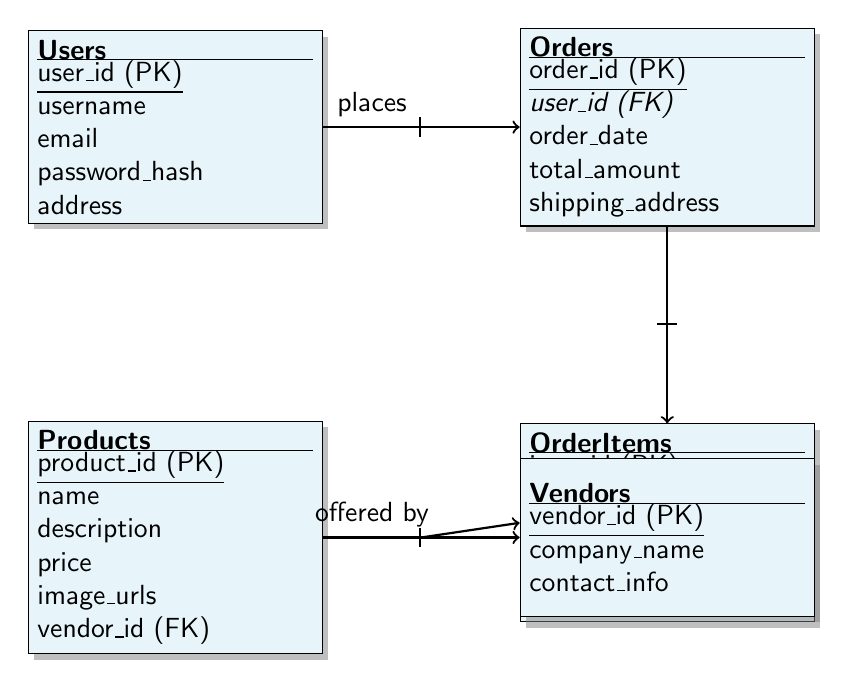
\begin{tikzpicture}[
    node distance=2.5cm,
    font=\sffamily,
    entity/.style={rectangle, draw, fill=SkyBlue!20, text width=3.5cm, minimum height=2cm, align=left, drop shadow},
    one/.style={-|, thick},
    many/.style={->, thick}
]

\node[entity] (user) {\textbf{Users} \\ \hrule \underline{user\_id (PK)} \\ username \\ email \\ password\_hash \\ address};
\node[entity, right=of user] (order) {\textbf{Orders} \\ \hrule \underline{order\_id (PK)} \\ \textit{user\_id (FK)} \\ order\_date \\ total\_amount \\ shipping\_address};
\node[entity, below=of order] (order_item) {\textbf{OrderItems} \\ \hrule \underline{item\_id (PK)} \\ \textit{order\_id (FK)} \\ \textit{product\_id (FK)} \\ quantity \\ price};
\node[entity, below=of user] (product) {\textbf{Products} \\ \hrule \underline{product\_id (PK)} \\ name \\ description \\ price \\ image\_urls \\ vendor\_id (FK)};
\node[entity, right=of product] (vendor) {\textbf{Vendors} \\ \hrule \underline{vendor\_id (PK)} \\ company\_name \\ contact\_info};

\draw[one] (user.east) -- node[above, midway] {places} ++(1.25,0) coordinate (t1);
\draw[many] (t1) -- (order.west);
\draw[one] (order.south) -- ++(0,-1.25) coordinate (t2);
\draw[many] (t2) -- (order_item.north);
\draw[one] (product.east) -- node[above, midway] {offered by} ++(1.25,0) coordinate (t3);
\draw[many] (t3) -- (vendor.west);
\draw[one] (product.east) -- ++(1.25,0) coordinate (t4);
\draw[many] (t4) -- (order_item.west);

\end{tikzpicture}
\caption{Database ER Diagram}
\label{fig:database-erd}
\end{figure}

\subsection{Physical Database Design}

**(PostgreSQL - User and Order Tables)**

```sql
CREATE TABLE users (
    user_id SERIAL PRIMARY KEY,
    username VARCHAR(255) UNIQUE NOT NULL,
    email VARCHAR(255) UNIQUE NOT NULL,
    password_hash VARCHAR(255) NOT NULL,
    address TEXT
);

CREATE TABLE orders (
    order_id SERIAL PRIMARY KEY,
    user_id INTEGER REFERENCES users(user_id) ON DELETE CASCADE,
    order_date TIMESTAMP DEFAULT CURRENT_TIMESTAMP,
    total_amount DECIMAL(10, 2) NOT NULL,
    shipping_address TEXT
);

CREATE TABLE order_items (
    item_id SERIAL PRIMARY KEY,
    order_id INTEGER REFERENCES orders(order_id) ON DELETE CASCADE,
    product_id INTEGER, -- Assuming product_id is from MongoDB
    quantity INTEGER NOT NULL,
    price DECIMAL(10, 2) NOT NULL
);
```

**(MongoDB - Product Collection)**  Schema will be flexible to accommodate various product attributes.

```json
{
  "product_id": 123,
  "name": "Example Product",
  "description": "A detailed description of the product...",
  "price": 99.99,
  "image_urls": ["url1.jpg", "url2.jpg"],
  "vendor_id": 456,
  "category": "Electronics",
  "specifications": {
    "size": "10x10",
    "weight": "1kg"
  }
}
```

\section{API Design and Integration}

\subsection{RESTful API Specification}

The APIs will follow RESTful principles, utilizing standard HTTP methods and JSON for data exchange.  Authentication will be handled via JWTs.

**Example Endpoint:**  `/products/{product_id}`

* **GET:** Retrieve product details.  Returns a JSON representation of the product.
* **PUT:** Update product details (requires vendor authentication).
* **DELETE:** Delete a product (requires vendor authentication).

**Example Response (GET /products/123):**

```json
{
  "product_id": 123,
  "name": "Example Product",
  "description": "A detailed description...",
  "price": 99.99,
  "image_urls": ["url1.jpg", "url2.jpg"],
  "vendor_id": 456
}
```

\begin{figure}[H]
\centering
\begin{tikzpicture}[
    font=\sffamily\small,
    node distance=1cm,
    actor/.style={rectangle, draw, fill=Azure!30, text width=2cm, text centered, rounded corners, drop shadow},
    service/.style={rectangle, draw, fill=LimeGreen!20, text width=2cm, text centered, rounded corners, drop shadow},
    db/.style={cylinder, shape border rotate=90, draw, fill=Thistle!40, text centered, drop shadow, minimum width=2cm, minimum height=1.2cm},
    lifeline/.style={dashed, thin, draw=gray},
    msg/.style={-Stealth, thick}
]

\node[actor] (client) at (0,0) {Client App};
\node[service] (api) at (3,0) {API Gateway};
\node[service] (catalog) at (6,0) {Catalog Service};
\node[db] (db) at (9,0) {Product Database};

\draw[lifeline] (client.south) -- ++(0,-4);
\draw[lifeline] (api.south) -- ++(0,-4);
\draw[lifeline] (catalog.south) -- ++(0,-4);
\draw[lifeline] (db.south) -- ++(0,-4);

\draw[msg] ($(client.south)+(0,-0.5)$) -- node[above] {1. GET /products/123} ($(api.south)+(0,-0.5)$);
\draw[msg] ($(api.south)+(0,-1)$) -- node[above] {2. Forward} ($(catalog.south)+(0,-1)$);
\draw[msg] ($(catalog.south)+(0,-1.5)$) -- node[above] {3. Query DB} ($(db.south)+(0,-1.5)$);
\draw[msg] ($(db.south)+(0,-2)$) -- node[above] {4. Product Data} ($(catalog.south)+(0,-2)$);
\draw[msg] ($(catalog.south)+(0,-2.5)$) -- node[above] {5. Response} ($(api.south)+(0,-2.5)$);
\draw[msg] ($(api.south)+(0,-3)$) -- node[above] {6. Product Data} ($(client.south)+(0,-3)$);

\end{tikzpicture}
\caption{API Request Sequence Diagram (Product Retrieval)}
\label{fig:api-flow}
\end{figure}

\subsection{API Security and Rate Limiting}

API security will be implemented using JWTs for authentication and authorization.  Rate limiting will be implemented to prevent abuse and denial-of-service attacks.  Input validation and sanitization will be performed on all API requests to prevent injection attacks.  HTTPS will be used for all communication to protect data in transit.  Regular security audits and penetration testing will be conducted to identify and address vulnerabilities.

\section{Security Architecture and Implementation}

\subsection{Security Requirements and Threat Model}

The security architecture will follow a layered approach, incorporating multiple security controls to protect against various threats.  A detailed threat model will be created, identifying potential threats and vulnerabilities.  Key security requirements include:

* **Authentication and Authorization:**  Secure user authentication using strong passwords and multi-factor authentication (MFA) where appropriate.  Role-based access control (RBAC) will be implemented to restrict access to sensitive data and functionalities.
* **Data Protection:** Data encryption at rest and in transit will be implemented to protect sensitive data.  Regular data backups will be performed to ensure data recovery in case of failure.
* **Input Validation and Sanitization:**  Strict input validation will be performed on all user inputs to prevent injection attacks.
* **Network Security:**  A firewall will be used to protect the platform's network infrastructure.  Intrusion detection and prevention systems (IDS/IPS) will be deployed to monitor and respond to security threats.
* **Regular Security Audits and Penetration Testing:**  Regular security audits and penetration testing will be conducted to identify and address vulnerabilities.

\begin{figure}[H]
\centering
\begin{tikzpicture}[
    font=\sffamily\small,
    node distance=0.8cm and 1.2cm,
    gate/.style={rectangle, draw, fill=red!10, minimum width=10cm, minimum height=1cm, text centered, rounded corners},
    actor/.style={rectangle, draw, fill=Azure!30, text centered, rounded corners, drop shadow},
    service/.style={rectangle, draw, fill=SkyBlue!20, text centered, rounded corners, drop shadow},
    arrow/.style={-Stealth, thick, draw=black!70}
]

\node[gate] (waf) at (0,0) {\textbf{Edge Protection}: WAF and DDoS Mitigation};
\node[gate, below=of waf] (ssl) {\textbf{Transport Layer}: SSL/TLS Termination};
\node[gate, below=of ssl] (authn) {\textbf{Authentication}: OAuth 2.0 / JWT Validation};
\node[gate, below=of authn] (authz) {\textbf{Authorization}: Rate Limiting and RBAC};
\node[service, below=1.2cm of authz] (backend) {Protected Backend Services};

\node[actor, above=1cm of waf] (user) {User};

\draw[arrow] (user) -- node[right] {HTTPS Request} (waf.north);
\draw[arrow] (waf.south) -- (ssl.north);
\draw[arrow] (ssl.south) -- (authn.north);
\draw[arrow] (authn.south) -- (authz.north);
\draw[arrow] (authz.south) -- node[right] {Authorized Request} (backend);

\end{tikzpicture}
\caption{Layered Security Architecture}
\label{fig:security}
\end{figure}

\section{Deployment and Infrastructure}

\subsection{Cloud Infrastructure Design}

The platform will be deployed on Amazon Web Services (AWS), leveraging its scalability and reliability.  A multi-availability zone (AZ) deployment will ensure high availability.  The architecture will utilize:

* **Load Balancers:**  Distribute traffic across multiple application servers.
* **Auto Scaling Groups:**  Automatically scale the number of application servers based on demand.
* **Containerization (Docker/Kubernetes):**  Package and deploy microservices in containers for improved portability and scalability.
* **Relational Database (RDS):**  Managed relational database service for PostgreSQL and MySQL.
* **NoSQL Database (DocumentDB):**  Managed NoSQL database service for MongoDB.
* **Message Broker (Amazon SQS/RabbitMQ):**  For asynchronous communication between microservices.
* **CloudWatch:**  For monitoring and logging.

\begin{figure}[H]
\centering
\begin{tikzpicture}[
    font=\sffamily\small,
    node distance=0.8cm and 1cm,
    server/.style={rectangle, draw, fill=gray!30, minimum height=1.5cm, minimum width=2.5cm, text centered, rounded corners, drop shadow},
    container/.style={rectangle, draw, fill=SkyBlue!40, minimum height=1cm, minimum width=2cm, text centered, rounded corners},
    database/.style={server, fill=Thistle!50},
    subnet/.style={rectangle, draw, fill=gray!10, rounded corners, inner sep=0.5cm, minimum height=4cm}
]

\node (internet) {Internet};
\node[server, below=1cm of internet] (lb) {Load Balancer};
\node[subnet, below=of lb, minimum width=9cm] (public_subnet) {};
\node[subnet, below=1.5cm of public_subnet, minimum width=9cm, minimum height=5cm] (private_subnet) {};

\node[above right] at (public_subnet.north west) {Public Subnet};
\node[above right] at (private_subnet.north west) {Private Subnet};

\node[server, align=center] (app1) at ($(private_subnet.center)+(-3,1)$) {Catalog Service\\(EC2)};
\node[container, below=0.1cm of app1] {Container};
\node[server, align=center] (app2) at ($(private_subnet.center)+(0,1)$) {Order Service\\(EC2)};
\node[container, below=0.1cm of app2] {Container};
\node[server, align=center] (app3) at ($(private_subnet.center)+(3,1)$) {Auth Service\\(EC2)};
\node[container, below=0.1cm of app3] {Container};

\node[database] (db-master) at ($(private_subnet.center)+(-1.5,-1.5)$) {Product DB (MongoDB)};
\node[database] (db-slave) at ($(private_subnet.center)+(1.5,-1.5)$) {Order DB (MySQL)};

\draw[-Stealth, thick] (internet) -- node[right, pos=0.4] {HTTPS Traffic} (lb);
\draw[-Stealth, thick] (lb) -- (public_subnet.north);
\draw[-Stealth, thick] ($(public_subnet.south)+(0,-0.75)$) -- (app1);
\draw[-Stealth, thick] ($(public_subnet.south)+(0,-0.75)$) -- (app2);
\draw[-Stealth, thick] ($(public_subnet.south)+(0,-0.75)$) -- (app3);
\draw[-Stealth, thick] (app1) -- (db-master);
\draw[-Stealth, thick] (app2) -- (db-slave);
\draw[<->, thick, dashed] (db-master) -- node[midway, below] {Replication} (db-slave);

\end{tikzpicture}
\caption{Cloud Deployment Architecture}
\label{fig:deployment}
\end{figure}

\section{Performance and Scalability}

Performance will be monitored through key performance indicators (KPIs) such as response time, throughput, and error rate.  Load testing will be conducted to ensure the platform can handle peak loads.  Scalability will be achieved through the use of cloud-native technologies, such as auto-scaling groups and containerization.  Database optimization techniques, such as indexing and query optimization, will be employed to improve database performance.  Caching mechanisms (Redis) will be implemented to reduce database load and improve response times.  Performance bottlenecks will be identified and addressed through continuous monitoring and performance tuning.

\section{Testing and Quality Assurance}

A comprehensive testing strategy will be implemented, including unit testing, integration testing, system testing, and user acceptance testing (UAT).  Automated testing will be used wherever possible to improve efficiency and reduce the risk of errors.  Test cases will be designed to cover all aspects of the platform's functionality, including both positive and negative scenarios.  Performance testing will be conducted to evaluate the platform's scalability and responsiveness under various load conditions.  Security testing will be performed to identify and address vulnerabilities.  The testing process will follow an agile methodology, with continuous integration and continuous delivery (CI/CD) pipelines to ensure rapid feedback and iterative improvements.

\section{Risk Assessment and Mitigation}

Several risks have been identified, including:

* **Technical Risks:**  Technology selection, integration challenges, and potential performance issues.
* **Schedule Risks:**  Delays in development, testing, or deployment.
* **Budget Risks:**  Cost overruns due to unforeseen circumstances.
* **Security Risks:**  Vulnerabilities in the platform's security architecture.

Mitigation strategies include:

* **Thorough planning and risk assessment:**  Identify and address potential risks early in the development process.
* **Agile development methodology:**  Allow for flexibility and adaptation to changing requirements.
* **Regular monitoring and communication:**  Track progress, identify potential issues, and communicate effectively with stakeholders.
* **Robust security measures:**  Implement security controls to protect against various threats.

\section{Implementation Roadmap and Timeline}

The project will be implemented in three phases:

* **Phase 1 (Months 1-2): Design and Development:**  Focus on designing the architecture, developing core services, and setting up the development environment.
* **Phase 2 (Months 3-4): Testing and Quality Assurance:**  Conduct thorough testing of all components and address any identified issues.
* **Phase 3 (Months 5-6): Deployment and Launch:**  Deploy the platform to the production environment and launch the platform.

\section{Monitoring and Maintenance}

The platform will be continuously monitored using CloudWatch.  Alerting mechanisms will be implemented to notify the operations team of any critical issues.  Regular maintenance tasks, such as software updates and database backups, will be performed to ensure the platform's stability and security.  Performance monitoring will be used to identify and address any performance bottlenecks.  A dedicated support team will be responsible for addressing user inquiries and resolving technical issues.

\section{Conclusion}

This document provides a comprehensive design for Project Phoenix, a robust and scalable e-commerce platform.  The microservices architecture, coupled with cloud-native technologies and a well-defined security strategy, will ensure the platform's success.  The implementation roadmap outlines a clear plan for development, testing, and deployment.  Continuous monitoring and maintenance will ensure the platform's long-term stability and performance.

\end{document}